\documentclass{article}
\usepackage{graphicx}

\title{Labwork 4: Threads}
\author{Nguyen Nhu Duy}
\date{}

\begin{document}

\maketitle

\section{Implementation}

The grayscale CUDA implementation from Labwork 3 was improved by using
2D blocks and a 2D grid. Each CUDA thread directly processes one image
pixel using its $(x,y)$ coordinates, instead of using a 1D index.

\section{2D Block Size Experiment}

Different 2D block sizes were tested, including $(8,8)$, $(16,16)$,
$(32,16)$, $(16,32)$, and $(32,32)$. The execution time was measured
using \texttt{time.time()}. A warm-up run was performed before timing,
and the reported execution time was calculated as the average of five runs.

The 2D implementation achieved average execution times from approximately
0.000156 s to 0.000256 s. Compared with the previous 1D implementation,
which required approximately 0.027--0.030 s, the 2D implementation was
about 105--192 times faster. The best result was obtained with a
$(16,16)$ block size at approximately 0.000156 s.

\begin{center}
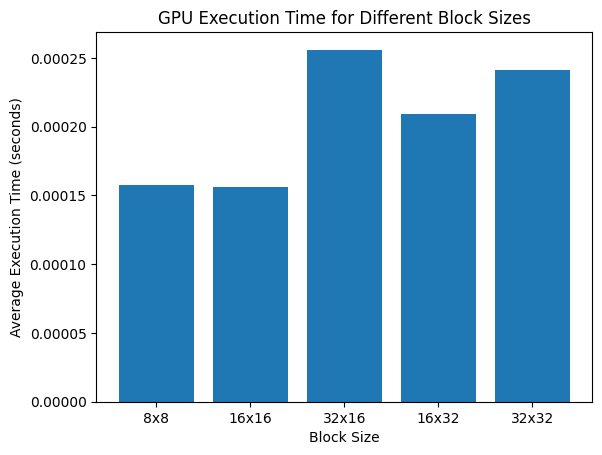
\includegraphics[width=0.8\textwidth]{block_size_speedup.png}
\end{center}

\end{document}